\documentclass[11pt]{article}

\usepackage[margin=1in]{geometry}
\usepackage{amsmath,amssymb,amsfonts}
\usepackage{algorithm}
\usepackage{algpseudocode}
\usepackage{graphicx}
\graphicspath{{figures/}{../results/figures/}}
\usepackage{booktabs}
\usepackage{hyperref}
\usepackage{float}

\title{A From-Scratch Implementation and Comparison of ISTA and FISTA for Lasso Regression}
\author{Yohannes T. Haile}
\date{\today}

\begin{document}
\maketitle

\begin{abstract}
This project implements the Iterative Shrinkage-Thresholding Algorithm (ISTA)
and the Fast Iterative Shrinkage-Thresholding Algorithm (FISTA) for the Lasso
regression problem. The objective, gradient, and proximal operator are derived
and implemented using NumPy. Experiments compare objective values, objective
gaps, and iteration counts on reproducible synthetic sparse-regression data.
Numerical results demonstrate that FISTA achieves faster convergence (108 iterations vs.\ 137 iterations for ISTA at tolerance $10^{-10}$) while obtaining the identical optimal objective value and sparse coefficient support.
\end{abstract}

\section{Introduction}
Many large-scale optimization problems combine a differentiable loss with a
nonsmooth regularizer. Lasso regression is a useful example because the
quadratic loss is smooth while the $\ell_1$ penalty promotes sparse solutions.
ISTA applies a proximal-gradient step, while FISTA accelerates this scheme
using an extrapolation sequence.

The principal reference is Beck and Teboulle's original FISTA paper:
\href{https://doi.org/10.1137/080716542}{A Fast Iterative Shrinkage-Thresholding
Algorithm for Linear Inverse Problems} (2009).

\section{Optimization Problem}
Let $X\in\mathbb{R}^{n\times p}$ be a design matrix, $y\in\mathbb{R}^n$ the
response, and $\beta\in\mathbb{R}^p$ the coefficient vector. We minimize
\begin{equation}
  \min_{\beta\in\mathbb{R}^p} F(\beta)
  = f(\beta)+g(\beta)
  = \frac{1}{2n}\|X\beta-y\|_2^2+\lambda\|\beta\|_1,
  \label{eq:lasso}
\end{equation}
where $\lambda\geq 0$. The function $f$ is convex and differentiable, and
$g(\beta)=\lambda\|\beta\|_1$ is convex but generally nondifferentiable.

\section{Gradient and Lipschitz Constant}
Expanding the quadratic loss,
\begin{align}
f(\beta)
&=\frac{1}{2n}(X\beta-y)^\top(X\beta-y)\\
&=\frac{1}{2n}\left(\beta^\top X^\top X\beta
-2y^\top X\beta+y^\top y\right).
\end{align}
Therefore,
\begin{equation}
\nabla f(\beta)=\frac{1}{n}X^\top(X\beta-y).
\label{eq:gradient}
\end{equation}
The gradient is Lipschitz continuous with constant
\begin{equation}
L=\frac{\|X^\top X\|_2}{n}=\frac{\|X\|_2^2}{n}.
\label{eq:lipschitz}
\end{equation}
A standard step size is $\alpha=1/L$.

\section{Proximal Operator and Soft-Thresholding}
For $\alpha>0$, the proximal operator of $\alpha g$ is
\begin{equation}
\operatorname{prox}_{\alpha g}(z)
=\arg\min_u\left\{\frac{1}{2}\|u-z\|_2^2+
\alpha\lambda\|u\|_1\right\}.
\end{equation}
The minimization separates by coordinate. For a scalar $z_i$, consider
\begin{equation}
\min_{u_i}\;\frac{1}{2}(u_i-z_i)^2+\alpha\lambda|u_i|.
\end{equation}
For $u_i>0$, the stationary condition gives $u_i=z_i-\alpha\lambda$;
for $u_i<0$, it gives $u_i=z_i+\alpha\lambda$. At zero, the subgradient
condition is satisfied when $|z_i|\leq\alpha\lambda$. Combining the cases gives
\begin{equation}
\operatorname{prox}_{\alpha g}(z)_i
=S_{\alpha\lambda}(z_i)
=\operatorname{sign}(z_i)\max(|z_i|-\alpha\lambda,0).
\label{eq:soft}
\end{equation}

\section{ISTA}
With $\alpha=1/L$, ISTA updates
\begin{equation}
\beta_{k+1}=
\operatorname{prox}_{g/L}\left(\beta_k-\frac{1}{L}\nabla f(\beta_k)\right),
\end{equation}
or, using soft-thresholding,
\begin{equation}
\beta_{k+1}=
S_{\lambda/L}\left(\beta_k-\frac{1}{L}\nabla f(\beta_k)\right).
\end{equation}

\begin{algorithm}[H]
\caption{ISTA for Lasso}
\begin{algorithmic}[1]
\Require $X,y,\lambda$, tolerance $\varepsilon$, maximum iterations $K$
\State Compute $L=\|X\|_2^2/n$ and initialize $\beta_0=0$
\For{$k=0,\ldots,K-1$}
  \State $u_k=\beta_k-\nabla f(\beta_k)/L$
  \State $\beta_{k+1}=S_{\lambda/L}(u_k)$
  \If{stopping criterion is satisfied}
    \State \textbf{break}
  \EndIf
\EndFor
\State \Return $\beta_{k+1}$
\end{algorithmic}
\end{algorithm}

\section{FISTA}
FISTA introduces an extrapolated point $z_k$ and scalar sequence $t_k$:
\begin{align}
\beta_{k+1}&=S_{\lambda/L}\left(z_k-\frac{1}{L}\nabla f(z_k)\right),\\
t_{k+1}&=\frac{1+\sqrt{1+4t_k^2}}{2},\\
z_{k+1}&=\beta_{k+1}+
\frac{t_k-1}{t_{k+1}}(\beta_{k+1}-\beta_k),
\end{align}
with $\beta_0=z_0$ and $t_0=1$.

\begin{algorithm}[H]
\caption{FISTA for Lasso}
\begin{algorithmic}[1]
\Require $X,y,\lambda$, tolerance $\varepsilon$, maximum iterations $K$
\State Compute $L=\|X\|_2^2/n$
\State Initialize $\beta_0=z_0=0$ and $t_0=1$
\For{$k=0,\ldots,K-1$}
  \State $\beta_{k+1}=S_{\lambda/L}(z_k-\nabla f(z_k)/L)$
  \State $t_{k+1}=(1+\sqrt{1+4t_k^2})/2$
  \State $z_{k+1}=\beta_{k+1}+\frac{t_k-1}{t_{k+1}}(\beta_{k+1}-\beta_k)$
  \If{stopping criterion is satisfied}
    \State \textbf{break}
  \EndIf
\EndFor
\State \Return $\beta_{k+1}$
\end{algorithmic}
\end{algorithm}

\section{Convergence Discussion}
Under standard assumptions for convex composite optimization, ISTA has an
$O(1/k)$ worst-case objective-suboptimality bound, while FISTA achieves
$O(1/k^2)$. These are theoretical bounds, not claims that each FISTA iteration
must decrease the objective. Standard FISTA is not necessarily monotone.

\section{Experimental Design}
The implementation generates synthetic data $y=X\beta^\star+\epsilon$ with a
sparse coefficient vector $\beta^\star$ and Gaussian noise $\epsilon$. The
experiments compare:
\begin{itemize}
  \item objective value versus iteration;
  \item objective gap relative to a high-accuracy reference value;
  \item iterations needed to reach a specified tolerance;
  \item estimated number of nonzero coefficients;
  \item sensitivity to predictor correlation.
\end{itemize}
For fair comparison, use the same data, regularization parameter, initialization,
Lipschitz constant, and stopping rule for both algorithms. State clearly how
the reference objective is computed; the lowest value from two finite runs is
only a practical reference, not a certified optimum.

\section{Results}
The numerical experiments were executed on synthetic sparse linear regression data
with $n=250$ observations, $p=500$ features, $s=15$ true nonzero coefficients, and noise
standard deviation $\sigma=0.1$. The regularization parameter was set to $\lambda=0.1$
and convergence tolerance $\varepsilon=10^{-10}$. The computed Lipschitz constant for
the gradient was $L = \|X\|_2^2 / n \approx 5.8827$.

Table~\ref{tab:results} summarizes the performance of ISTA and FISTA. Both methods converged
successfully to the same optimal objective value ($F \approx 2.09053382$) and recovered
16 nonzero coefficients ($|\beta_j| > 10^{-8}$). FISTA required 108 iterations to achieve
convergence compared to 137 iterations for ISTA, demonstrating the acceleration achieved
by the Nesterov-style momentum sequence.

\begin{table}[H]
\centering
\begin{tabular}{lrrrr}
\toprule
Method & Iterations & Final objective & Nonzero coefficients & Converged\\
\midrule
ISTA  & 137 & 2.09053382 & 16 & Yes \\
FISTA & 108 & 2.09053382 & 16 & Yes \\
\bottomrule
\end{tabular}
\caption{Numerical performance of ISTA and FISTA on synthetic sparse regression data ($n=250$, $p=500$, $s=15$, $\lambda=0.1$, $\varepsilon=10^{-10}$).}
\label{tab:results}
\end{table}

Figure~\ref{fig:gap} presents the objective gap $F(\beta_k) - F_{\mathrm{ref}}$ across iterations
on a logarithmic scale, where $F_{\mathrm{ref}}$ is the minimum objective value obtained across
both runs. FISTA demonstrates a noticeably steeper rate of convergence.
Figure~\ref{fig:objective} shows the raw objective values as a function of iteration count.

\begin{figure}[H]
\centering
\IfFileExists{figures/objective_gap.png}{%
  \includegraphics[width=0.85\textwidth]{figures/objective_gap.png}%
}{%
  \includegraphics[width=0.85\textwidth]{../results/figures/objective_gap.png}%
}
\caption{Objective gap $F(\beta_k) - F_{\mathrm{ref}}$ by iteration for ISTA and FISTA.}
\label{fig:gap}
\end{figure}

\begin{figure}[H]
\centering
\IfFileExists{figures/objective_values.png}{%
  \includegraphics[width=0.85\textwidth]{figures/objective_values.png}%
}{%
  \includegraphics[width=0.85\textwidth]{../results/figures/objective_values.png}%
}
\caption{Objective values by iteration for ISTA and FISTA.}
\label{fig:objective}
\end{figure}

\section{Limitations and Future Work}
The current experiments are synthetic and do not exactly reproduce every
numerical experiment in the original paper, which studies linear inverse
problems. A closer reproduction should match a specific published experiment's
data, parameter choices, initialization, stopping criteria, and reported
metrics. Extensions include monotone FISTA, backtracking line search, restart
schemes, and systematic variation of sample size, feature count, and
correlation.

\section{Conclusion}
This project provides a transparent implementation of proximal-gradient
optimization for Lasso and a reproducible comparison of ISTA and FISTA.
The numerical experiments confirm that FISTA accelerates convergence, reaching
the tolerance stopping criterion in 108 iterations compared to 137 for ISTA,
while both methods converge to identical final objective values and sparse support.

\begin{thebibliography}{9}
\bibitem{beckteboulle2009}
A. Beck and M. Teboulle,
\emph{A Fast Iterative Shrinkage-Thresholding Algorithm for Linear Inverse Problems},
SIAM Journal on Imaging Sciences, 2(1), 183--202, 2009.
\href{https://doi.org/10.1137/080716542}{doi:10.1137/080716542}.
\end{thebibliography}

\end{document}
